%%%%%%%%%%%%%%%%%%%%%%%%%%%%%%%%%%%%%%%%%
% Beamer Presentation
% LaTeX Template
% Version 1.0 (10/11/12)
%
% This template has been downloaded from:
% http://www.LaTeXTemplates.com
%
% License:
% CC BY-NC-SA 3.0 (http://creativecommons.org/licenses/by-nc-sa/3.0/)
%
%%%%%%%%%%%%%%%%%%%%%%%%%%%%%%%%%%%%%%%%%

%----------------------------------------------------------------------------------------
%	PACKAGES AND THEMES
%----------------------------------------------------------------------------------------

\documentclass[9pt]{beamer}
\usepackage{CJK}
\usepackage{ctex}
\usepackage{graphicx}
\usepackage{subfigure}
\usepackage{longtable}
\usepackage{rotating}
\usepackage{multirow}
\usepackage{algorithm}
\usepackage{algorithmic}
\usepackage{mathtools}
\usepackage{animate}
\usepackage{amsthm, amsmath}
%\usepackage{media9}
%% A LATEX package for embedding interactive Adobe Flash (SWF) and 3D files (Adobe U3D & PRC) as well as video and sound files or streams (FLV, MP4/H.246, MP3) into PDF documents with Adobe Reader-9/X
%compatibility.
\renewcommand{\algorithmicrequire}{\textbf{Input:}}   %Use Input in the format of Algorithm
\renewcommand{\algorithmicensure}{\textbf{Output:}}  %UseOutput in the format of Algorithm
\newcommand{\e}[1]{\ensuremath{\times 10^{#1}}}
%\mode<presentation>{\usetheme{Madrid}}

\mode<presentation> {

% The Beamer class comes with a number of default slide themes
% which change the colors and layouts of slides. Below this is a list
% of all the themes, uncomment each in turn to see what they look like.

%\usetheme{default}
%\usetheme{AnnArbor}
%\usetheme{Antibes}
%\usetheme{Bergen}
%\usetheme{Berkeley}
%\usetheme{Berlin}
%\usetheme{Boadilla}
%\usetheme{CambridgeUS}
%\usetheme{Copenhagen}
%\usetheme{Darmstadt}
%\usetheme{Dresden}
%\usetheme{Frankfurt}
%\usetheme{Goettingen}
%\usetheme{Hannover}
%\usetheme{Ilmenau}
%\usetheme{JuanLesPins}
%\usetheme{Luebeck}
\usetheme{Madrid}
%\usetheme{Malmoe}
%\usetheme{Marburg}
%\usetheme{Montpellier}
%\usetheme{PaloAlto}
%\usetheme{Pittsburgh}
%\usetheme{Rochester}
%\usetheme{Singapore}
%\usetheme{Szeged}
%\usetheme{Warsaw}

% As well as themes, the Beamer class has a number of color themes
% for any slide theme. Uncomment each of these in turn to see how it
% changes the colors of your current slide theme.

%\usecolortheme{albatross}
\usecolortheme{beaver}
%\usecolortheme{beetle}
%\usecolortheme{crane}
%\usecolortheme{dolphin}
%\usecolortheme{dove}
%\usecolortheme{fly}
%\usecolortheme{lily}
%\usecolortheme{orchid}
%\usecolortheme{rose}
%\usecolortheme{seagull}
%\usecolortheme{seahorse}
%\usecolortheme{whale}
%\usecolortheme{wolverine}

%\setbeamertemplate{footline} % To remove the footer line in all slides uncomment this line
%\setbeamertemplate{footline}[page number] % To replace the footer line in all slides with a simple slide count uncomment this line

%\setbeamertemplate{navigation symbols}{} % To remove the navigation symbols from the bottom of all slides uncomment this line
}

\usepackage{graphicx} % Allows including images
\usepackage{booktabs} % Allows the use of \toprule, \midrule and \bottomrule in tables
\begin{document}
\begin{CJK*}{GBK}{kai}
%----------------------------------------------------------------------------------------
%	TITLE PAGE
%----------------------------------------------------------------------------------------

\title[Machine Learning]{Logistic Regression} % The short title appears at the bottom of every slide, the full title is only on the title page

\author{Kun He (����)} % Your name
%\logo{%
%   
\includegraphics[scale=.2]{logo.pdf}\hspace*{4.75cm}~%
%   
\includegraphics[scale=.2]{logo.jpg}\hspace*{0.75cm}%
%   }
%\pgfdeclareimage[width=1cm]{hust}{logo.pdf}
%\logo{\pgfuseimage{hust}{\vspace{-10pt}}}
\titlegraphic{
\includegraphics[width=1.3cm]{logo.pdf}}
\institute[JHL, HUST] % Your institution as it will appear on the bottom of every slide, may be shorthand to save space
{
	Data Mining and Machine Learning Lab\\
	(John Hopcroft Lab)\\
	Huazhong University of Science \& Technology \\ % Your institution for the title page
	\medskip
	\textit{brooklet60@hust.edu.cn} % Your email address
}

\date{2022��5��} % Date, can be changed to a custom date
%====================================================
\frame{\titlepage}

\frame{\frametitle{Table of contents}\tableofcontents}

\AtBeginSection[]
{
\begin{frame}{Table of Contents}
\tableofcontents[currentsection]
\end{frame}
}

%------------------------------------------------
%------------------------------------------------

\section{Introduction}
%------------------------------------------------
\subsection{Basic idea}
\begin{frame}
	\frametitle{Basic idea}
	
	\begin{figure}[h]
		\centering
		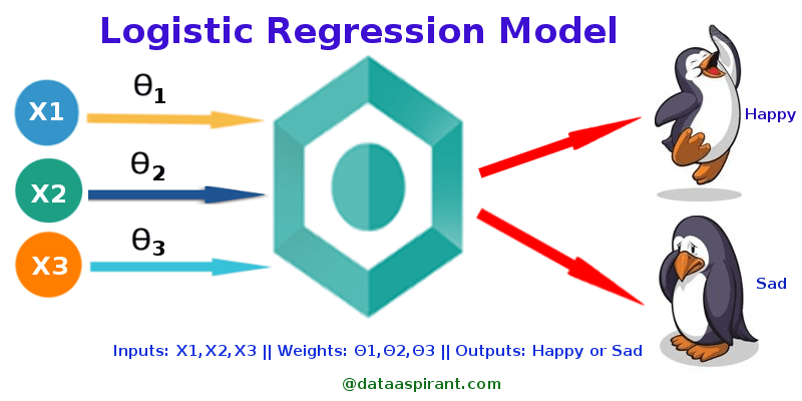
\includegraphics[scale=0.3]{4.png}
		\caption{Logistic regression is a classic machine learning algorithm used for classification task. As shown in the picture, we first feed the data, the inputs to the model, and the model gives us its classification result.
		}
	\end{figure}
	
\end{frame}
%------------------------------------------------
\begin{frame}
\frametitle{Basic idea}
\begin{itemize}
\item Logistic Regression is the discriminative counterpart to the Gaussian Naive Bayes (Naive Bayes for continuous features).
\item  Machine learning algorithms can be (roughly) categorized into two categories:\\
 a) \textbf{Generative} algorithms, that estimate $P(x_i,y)$ (often they model $P(x_i|y)$ and $P(y)$ separately).\\
 b) \textbf{Discriminative} algorithms, that model $P(y|x_i)$
 \item The Naive Bayes algorithm is generative. It models $P(x_i|y)$ and makes explicit assumptions on its distribution (e.g. categorical, multinomial, Gaussian, ...). The parameters of this distributions are estimated with MLE or MAP. 
\end{itemize}

Recall: 

1) Bayesian Rule:
\[p(Y|X) = \frac{p(X|Y)p(Y)}{p(X)}\]
~~

2) Bayesian Classification:
\[ \operatorname*{argmax}_{y} p(y)\prod_{i=1}^{n}p(x_{i} | y,\theta) = \operatorname*{argmax}_{y} [log(p(y)) + \sum_{i=1}^{n}log(p(x_{i} | y,\theta))] \]
\end{frame}
%------------------------------------------------
\begin{frame}
	\frametitle{Basic idea}
	\begin{itemize}
		\item We showed previously that for the Gaussian Naive Bayes 
		$P(y|x_i)=\frac{1}{1+e^{-y(w^Tx_i+b)}}$ 
		for $y\in \{+1,-1\}$ for specific vectors $w$ and $b$ that are uniquely determined through the particular choice of $P(x_i|y)$.
		\item Logistic Regression is often referred to as the discriminative counterpart of Naive Bayes. Here, we model $P(y|x_i)$ and assume that it takes on exactly this form
		$$P(y|x_i)=\frac{1}{1+e^{-y(w^Tx_i+b)}}$$ 
	\item The logistic (or sigmoid function):
	\end{itemize}
	\begin{figure}[h]
	\centering	
	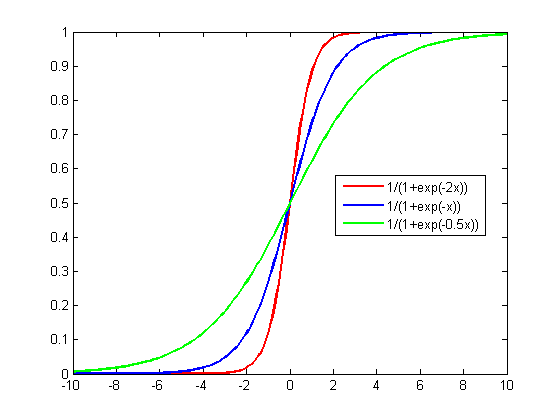
\includegraphics[scale=0.4]{sigmoidFunction.png}\end{figure}
\end{frame}

%------------------------------------------------
\begin{frame}
	\frametitle{Basic idea}
	\begin{itemize}
		\item We make assumptions on  $P(x_i|y)$, e.g. it could be Gaussian or Multinomial. Ultimately it doesn't matter, because we estimate the vector $w$ and $b$ directly with MLE or MAP to maximize the conditional likelihood of $\prod_i P(y_i|x_i;w,b)$.
		\item Throughout this lecture we absorbed the parameter b into w through an additional constant dimension (similar to the Perceptron).
	\end{itemize}
~~

\[P(y|X)=\frac{1}{1+e^{-y(w^TX)}}\]
\end{frame}
%------------------------------------------------
\subsection{Maximum likelihood estimate (MLE)}
\begin{frame}
	\frametitle{MLE for Logistic Regression}
	\begin{itemize}
		\item In MLE we choose parameters that \textbf{maximize the conditional likelihood}. The conditional data likelihood $P(Y|X,w)$ is the probability of the observed values $Y \in R^n $ in the training data conditioned on the feature values $x_i$. Note that $X=[x_1,��,x_i,��,x_n] \in R^{d\times n}$. We choose the parameters that maximize this function and we assume that the $y_i$'s are independent given the input features $x_i$ and $w$.
	\end{itemize}
	\begin{figure}[h]
	\centering
	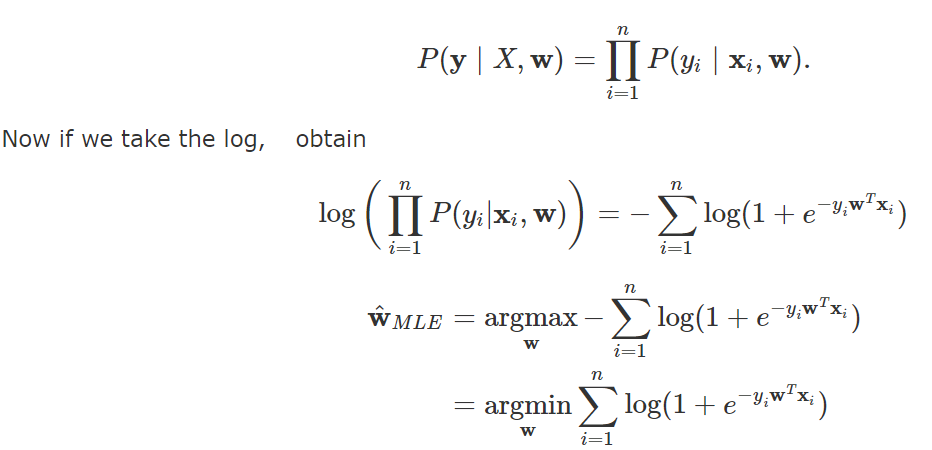
\includegraphics[scale=0.4]{MLE.png}		
	\end{figure}
\end{frame}

%------------------------------------------------
\begin{frame}
	\frametitle{MLE for Logistic Regression}
	\begin{figure}[h]
		\centering
		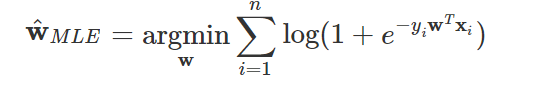
\includegraphics[scale=0.5]{MLE2.png}	
		\end{figure}
	\begin{itemize}
	\item We need to estimate the parameters $w$. To find the values of the parameters at minimum, we can try to find solutions for 
	$\nabla_w \sum_i^n log(1+e^{y_iw^Tx_i}) = 0$.
	\item This equation has no closed form solution, so we will use Gradient Descent on the negative log likelihood
  \end{itemize}	

  	\begin{figure}[h]
  	\centering
  	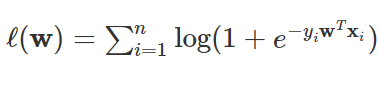
\includegraphics[scale=0.5]{MLENegLogLikelihood.png}	
  \end{figure}
\end{frame}
%------------------------------------------------
\begin{frame}
	\frametitle{1-D Example}
	Consider a 1D problem, with positive class marked as pluses and negative as circles.
	\begin{figure}[h]
		\centering
		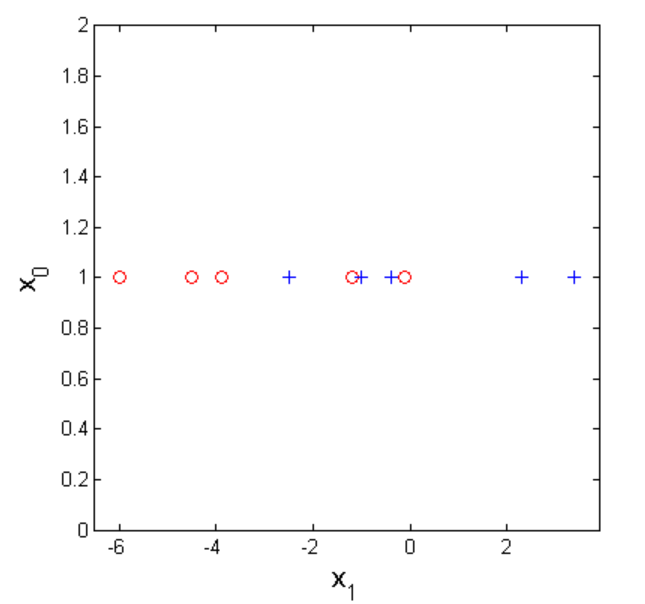
\includegraphics[scale=0.25]{1DExample.png}
		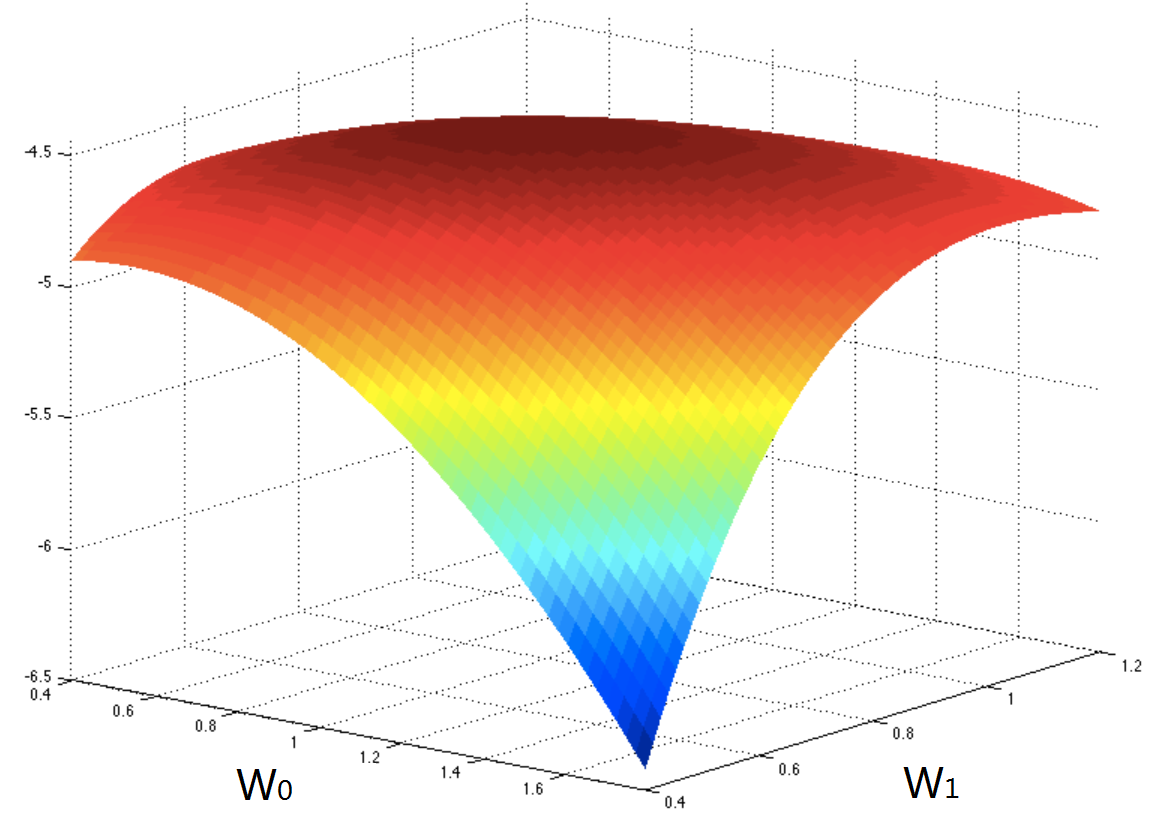
\includegraphics[scale=0.2]{1DLogLikelihood.png}
		\caption{(a) Dataset. Vertical axis is the constant feature $X_0 =1$. (b) Log likelihood.}	
	\end{figure}
	\begin{itemize}
		\item This log likelihood function is shown below in the space of the two parameters 
		($w_0,w_1$), with the maximum at 
		($w_0 =1$ and $w_1 = 0.7$).  
	\end{itemize}	
\end{frame}
%------------------------------------------------
\begin{frame}
	\frametitle{1-D Example}
 
	\begin{figure}[h]
		\centering
		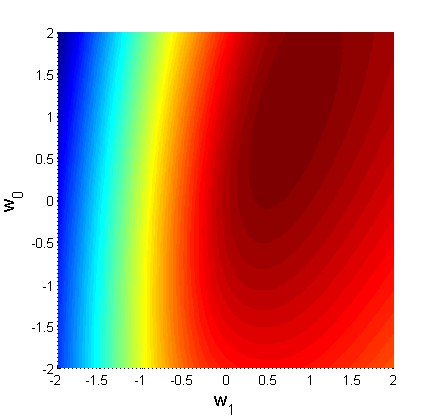
\includegraphics[scale=0.2]{1DHeatmap.png}
		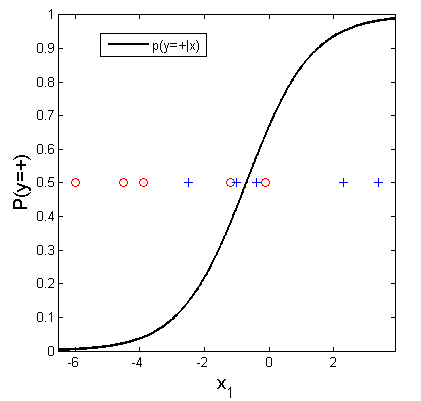
\includegraphics[scale=0.2]{1DSolution.png}		
		
		\caption{(a) Log likelihood heat map for dataset above. (b) The MLE solution.}	
	\end{figure}
	\begin{itemize}
		\item Here are the plots of the contributions of each example to the objective above.  
	\end{itemize}
	\begin{figure}[h]
	\centering
	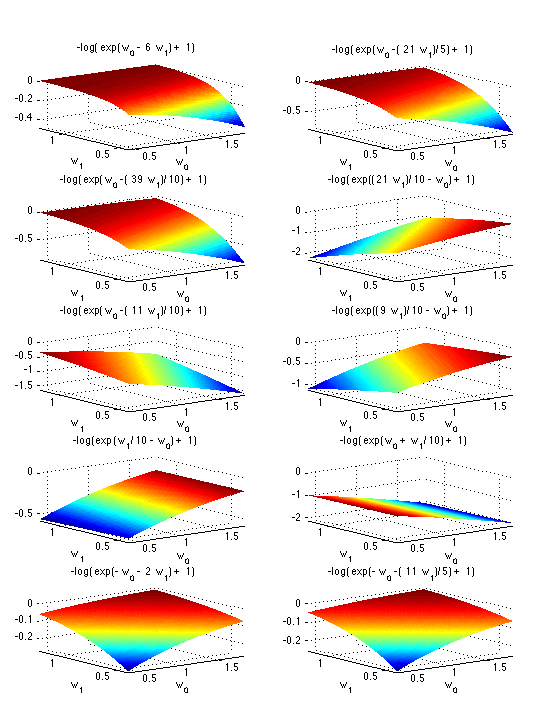
\includegraphics[scale=0.25]{1DeachContribution.png}
	%\caption{A plot of each example's contribution.}	
    \end{figure}	
\end{frame}


%------------------------------------------------
\begin{frame}
	\frametitle{2-D Example}
	Consider a 2D problem, with positive class marked as pluses and negative as circles. 
	\begin{figure}[h]
		\centering
		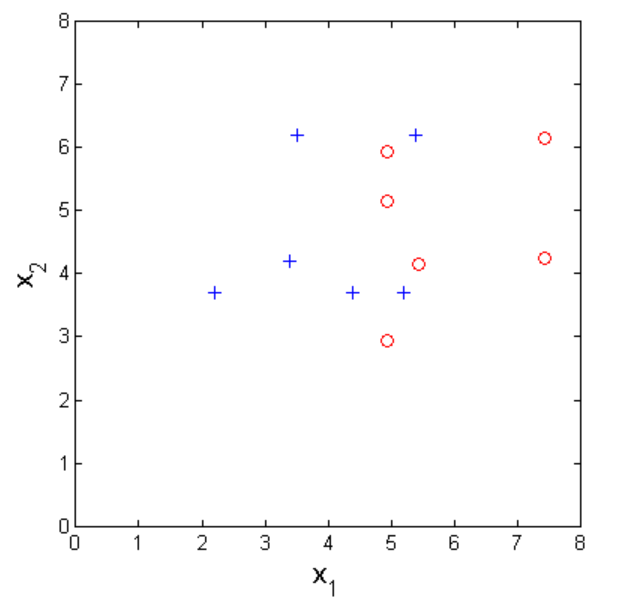
\includegraphics[scale=0.25]{2DExample.png}
		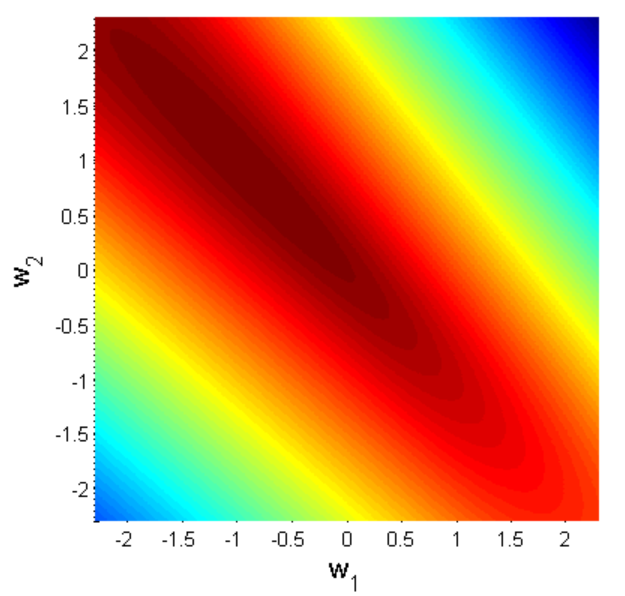
\includegraphics[scale=0.25]{2DLogLikelihood.png}
		\caption{(a) Dataset.  (b) Log likelihood function with the ($w_1,w_2$) be maximum at ($-0.81,0.81$).}	
	\end{figure}
\end{frame}

%------------------------------------------------
\begin{frame}
	\frametitle{1-D Example}
	
	\begin{figure}[h]
		\centering
		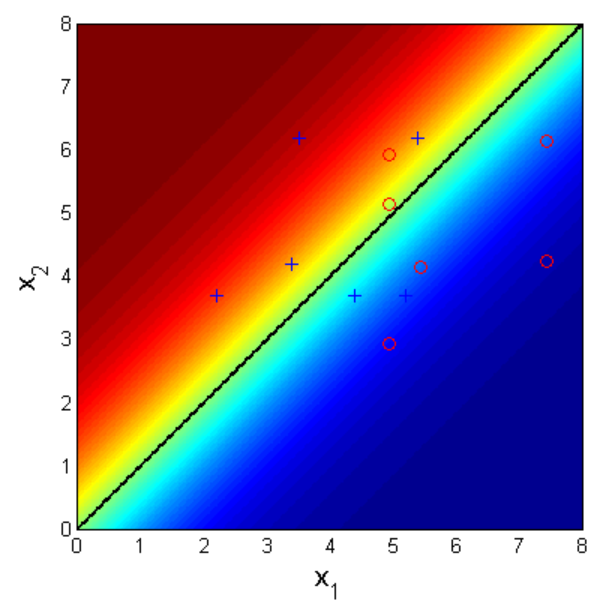
\includegraphics[scale=0.25]{2DSolution.png}		
		\caption{The MLE solution is displayed below, where the red color indicates high probability of positive class. The black line shows the decision boundary learned by MLE.}	
	\end{figure}

\textbf{Linear Decision Boundary}.    Why is the boundary linear? Consider the condition that holds at the boundary:
	\begin{figure}[h]
		\centering
		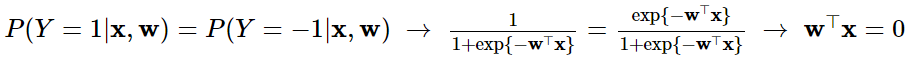
\includegraphics[scale=0.35]{LinearBoundary.png}
		%\caption{A plot of each example's contribution.}	
	\end{figure}	
For the toy problem above, the optimal 
$w$ is $(-0.81,0.81)$, so solving 
$w^Tx = 0.81 x_1 + 0.81 x_2 = 0$ we get the line $x_1 = x_2$.
\end{frame}


%------------------------------------------------

\subsection{Maximum a Posteriori (MAP) Estimate}
\begin{frame}
	\frametitle{MAP for Logistic Regression}
	\begin{itemize}
		\item In the MAP estimate we treat $w$ as a random variable and can specify a prior belief distribution over it. We assume a prior: $w\sim N(0,\sigma^2I)$. This is the Gaussian approximation for Logistic Regression.
		\item Our goal in MAP is to find the most likely model parameters given the data, i.e., the parameters that \textbf{maximize the posterior}.
	\end{itemize}
   \[ P(w|D) =  \frac{P(D|w)P(w)}{P(D)} \propto P(D|w)P(w)\]
   
   \[ P(w|D) = P(w|X,y) \propto P(X,y|w)P(w) \]
   \[~~~~~~~~~~~~~~~~~~~~~~~~~~ = P(y|X,w) P(X,w) P(w)
   \propto P(y|X,w)P(w) \]
   \[\hat{w}_{MAP} = \operatorname*{argmax}_w 
   log(P(y|X,w)P(w))
   \]
   \[ 
   ~~~~~~~~~~~~~~~~~~~~~~~~~~~~ 
   = \operatorname*{argmin}_{w} 
   \sum_{i=1}^n log(1+e^{y_iw^Tx_i})+ \lambda w^Tw
   \]

%	\begin{figure}[h]
%		\centering
%		\includegraphics[scale=0.45]{MAP.png}	
%	\end{figure}
	\begin{itemize}
	\item Here $\lambda=\frac{1}{2\sigma^2}$. Once again, this function has no closed form solution, but we can use Gradient Descent on the negative log posterior to find the optimal parameters.
	\end{itemize}
	\begin{figure}[h]
	\centering
	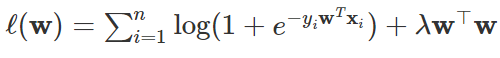
\includegraphics[scale=0.45]{negLogPosterior.png}	
    \end{figure}
\end{frame}


%------------------------------------------------

\subsection{Summary}
\begin{frame}
	\frametitle{Summary}
		\begin{itemize}
		\item Logistic Regression is the discriminative counterpart to Naive Bayes. 
		\item In Naive Bayes, we first model $P(x|y)$ for each label $y$, and then obtain the decision boundary that best discriminates between these two distributions. 
		\item In Logistic Regression we do not attempt to model the data distribution $P(x|y)$, instead, we model $P(y|x)$ directly. 
		\item We assume the same probabilistic form $P(y|x_i) = \frac{1}{1+e^{y(w^Tx_i+b)}}$ , but we do not restrict ourselves in any way by making assumptions about $P(x|y)$ (in fact it can be any member of the Exponential Family). 
		\item This allows logistic regression to be more flexible, but such flexibility also requires more data to avoid overfitting. 
		\item Typically, in scenarios with little data and if the modeling assumption is appropriate, Naive Bayes tends to outperform Logistic Regression. However, as data sets become large logistic regression often outperforms Naive Bayes, which suffers from the fact that the assumptions made on $P(x|y)$ are probably not exactly correct. 
		\item If the assumptions hold exactly, i.e. the data is truly drawn from the distribution that we assumed in Naive Bayes, then Logistic Regression and Naive Bayes converge to the exact same result in the limit (but NB will be faster).
	\end{itemize}
 
\end{frame}

%------------------------------------------------

 
\begin{frame}
	\frametitle{Naive Bayes vs. Logistic Regression}
	Let's consider the differences between the approaches:
	
	\begin{figure}[h]
		\centering	
		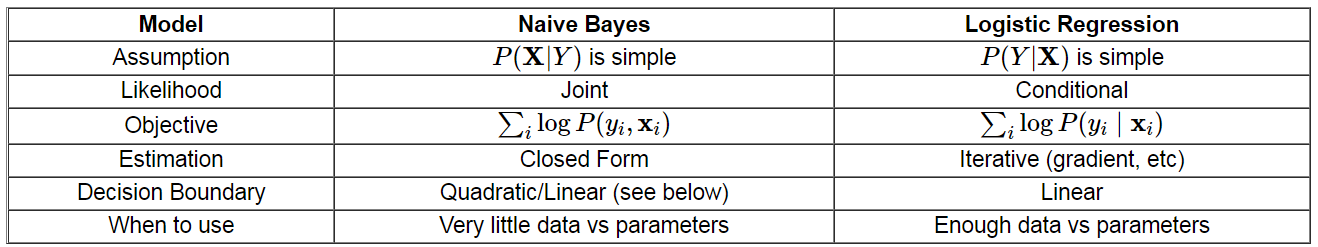
\includegraphics[scale=0.35]{NBvsLR.png}		\end{figure}
	
\end{frame}




%------------------------------------------------
\section{Further Discussion}
\subsection{The Function}
\begin{frame}
\frametitle{Introduction}
\begin{block}{Basic idea:}
	\begin{itemize}
		\item $f(z)=h_{\theta}(x)=sigmoid(z)=\frac{1}{1+e^{-z}}$
		\item Output = 0 or 1
		\item $Hypothesis \longrightarrow z=w^Tx+b$
	\end{itemize}
\end{block}
We usually attach the sigmoid function to the end of the model, it gives us the probability of the label being 1
\begin{figure}[h]
	\centering
	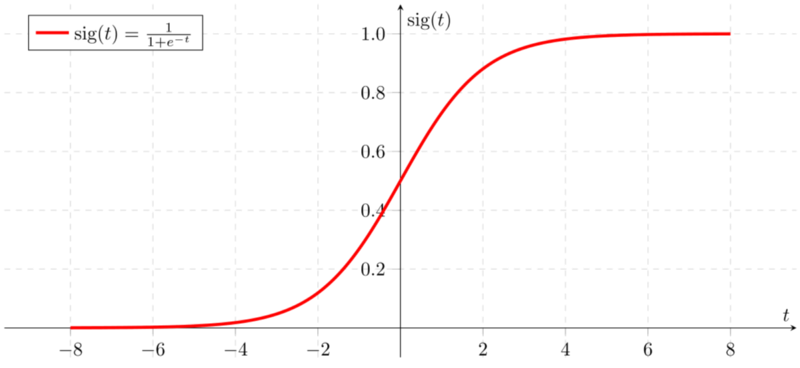
\includegraphics[scale=0.35]{5.png}
	\caption{If ��t�� goes to infinity, y(predicted) will become 1 and if ��t�� goes to negative infinity, y(predicted) will become 0.	
	}
\end{figure}
\end{frame}


\subsection{Loss Function}
\begin{frame}
	\frametitle{Loss Function}
	Predicted Probability:
	$$
	P(y=1|x)=h_\theta(x)=\frac1{1+e^{(-\theta^Tx})}=\sigma (\theta^Tx)\eqno{(1)}
	$$
	$$
	P(y=0|x)=1-P(y=1|x)=1-h_\theta(x)\eqno{(2)}
	$$
	Combined (1).(2):
	$$
	P(y|x;\theta)=(h_\theta(x))^y(1-h_\theta(x))^{1-y^{\color{red}\text{y stands for the labels, being 0 or 1}}}\eqno{(3)}
	$$
	
	Using maximum likelihood estimation(MLE) according to the $m$ given samples:
	$$
	L(\theta)=\prod^m_{i=1}P(y^{(i)}|x^{(i)};\theta)=\prod^m_{i=1}(h_\theta(x^{(i)}))y^{(i)}(1-h_\theta(x^{(i)}))^{1-y^{(i)}} \eqno{(6)}
	$$
	$$
	\longrightarrow \ell(\theta)=\log L(\theta)=\sum^m_{i=1}(y^{(i)}\log h_\theta(x^{(i)})+(1-y^{(i)})\log (1-h_\theta(y^{(i)})))\eqno{(7)}
	$$
	
	$$
	J(\theta)=-\frac{1}{m}\ell(\theta)\eqno{\color{red}\text{$J(\theta)$ is the desired loss function
	}}
	$$
	
\end{frame}
%%------------------------------------------------
\subsection{Regularization}
\begin{frame}
\frametitle{Regularization}
\begin{block}{Basic idea}
	\begin{itemize}
		\item L2$$
		J(\theta)=\frac{1}{2m}[\sum^m_{i=1}(h_\theta(x^{(i)}))^2+\lambda\sum^n_{j=1}\theta^2_j] \eqno{(8)}
		$$
		\item Regularization : prevent the weights from getting too large
		\item Regularization can avoid overfitting to some extent through the restraint of weights
	\end{itemize}
\end{block}
\end{frame}

\begin{frame}
\frametitle{Regularization}
\begin{figure}[h]
	\centering
	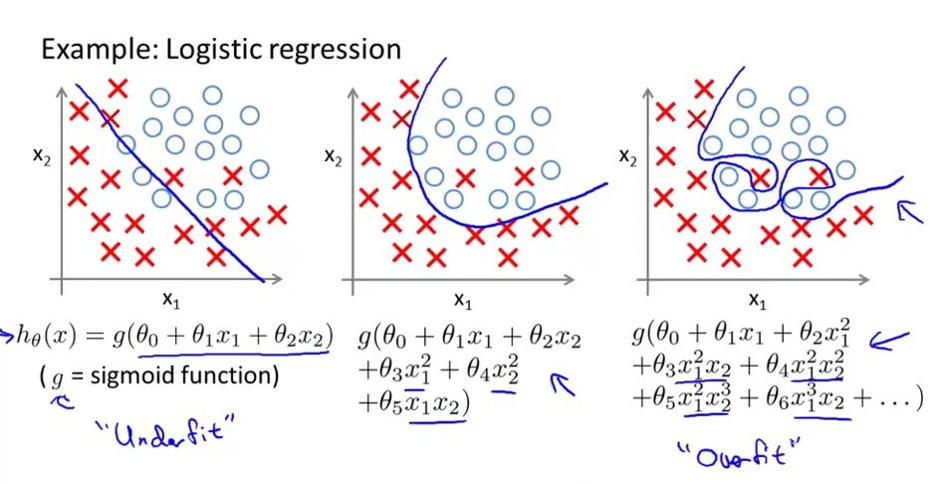
\includegraphics[scale=0.4]{6.png}
	\caption{Underfitting/overfitting
	}
\end{figure}
\end{frame}


\begin{frame}
\frametitle{Regularization}
Classification task through Logistic Regression
\begin{figure}[h]
	\centering
	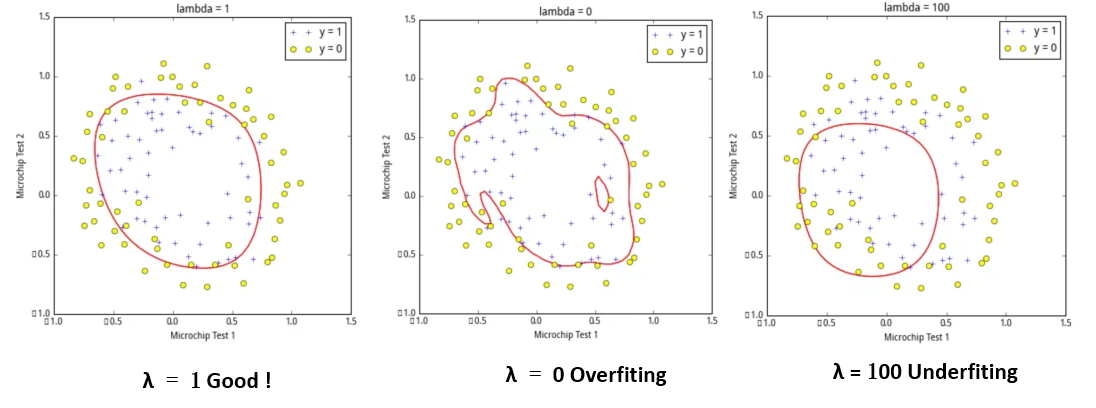
\includegraphics[scale=0.3]{7.png}
	\caption{Two-class classification when �� has different values
	}
\end{figure}
\end{frame}


\subsection{Weights Learning of LR}
\begin{frame}
\frametitle{Gradient Descent}
\begin{figure}[h]
	\centering
	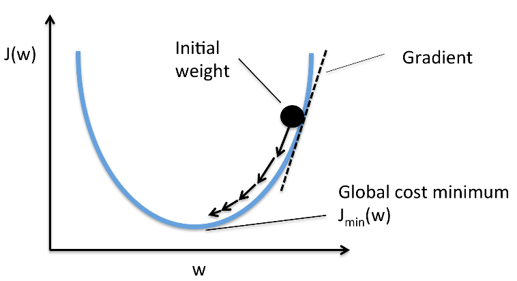
\includegraphics[scale=0.7]{8.png}
\end{figure}
\begin{figure}[h]
	\centering
	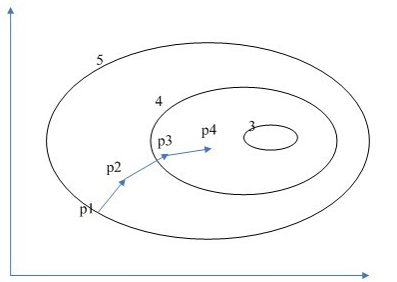
\includegraphics[scale=0.7]{9.png}
\end{figure}
\end{frame}
\begin{frame}
\frametitle{Gradient Descent}
$$
J(\theta)=-\sum^m_{i=1}(y^{(i)}\log h_\theta(x^{(i)})+(1-y^{(i)})\log (1-h_\theta(y^{(i)})))\eqno{(9)}
$$
$$\downarrow$$
Partial derivative:
$$\frac{\partial J(\theta)}{\partial \theta_j}=\sum_ix_j^{(i)}(h_\theta(x^{(i)})-y^{(i)})$$
$$\downarrow$$
Weights update:
$$\theta_j=\theta_j-\alpha\frac{\partial J(\theta)}{\partial J(\theta_j)}$$
\end{frame}

\section{Logistic Regression vs Naive Bayes}
\subsection{Comparison}
\begin{frame}
	\frametitle{Comparison}
	\begin{block}{Generative vs. Discriminative}
		\begin{itemize}
			\item Machine learning algorithms can be (roughly) categorized into two categories:
			\item Generative algorithms, that estimate $P(x_i,y)$ (often they model $P(x_i|y)$ and $P(y)$ separately).
			\item Discriminative algorithms, that model $P(y|x_i)$
		\end{itemize}
	\end{block}
1. The Naive Bayes algorithm is generative. ($p(y),p(x|y) \rightarrow p(y|x)$)
$$
P(y|x)=\frac{p(x,y)}{\prod_yp(x,y)}=\frac{p(y)p(x|y)}{\prod_yp(y)p(x|y)}
$$

2. Logistic Regression is discriminative. (Gradient descent$\rightarrow w$)
$$
P(y|x_i)=\frac1{1+e^{-y(w^Tx_i+b)}}
$$
\end{frame}
%%------------------------------------------------
%\section{Reference}
%------------------------------------------------
%\begin{frame}
%\frametitle{Reference}
%\begin{thebibliography}{4}
%\bibitem{LS-SPH} F. Zou, C. Liu, H. Ling, H. Feng, L. Yan, and D. Li, "Least square regularized spectral hashing for similarity search," Signal Processing, vol. 93, pp. 2265-2273, 2013. (SCI,EI)
%\bibitem{KMFH} F. Zou, Y. Chen, J. Song, K. Zhou, Y. Yang, and N. Sebe, "Compact image fingerprint via multiple kernel hashing," IEEE Transactions on Multimedia, vol. 17, pp. 1006-1018, 2015. (SCI,EI)
%\bibitem{KNPH} C. Liu, H. Ling, F. Zou, L. Yan, Y. Wang, H. Feng, et al., "Kernelized neighborhood preserving hashing for social-network-oriented digital fingerprints," IEEE Transactions on Information Forensics and Security, vol. 9, pp. 2232-2247, 2014. (SCI,EI)
%\bibitem{DTSH} Liu, Yu; Song, Jingkuan; Zhou, Ke; Yan, Lingyu; Liu, Li; Zou, Fuhao; Shao, Ling, "Deep Self-taught Hashing for Image Retrieval," IEEE Tra
%\bibitem{DeepFace} Fuhao Zou, Fan Yang, Wei Chen,Kai Lia, Jingkuan Song, Jingcai Chen, Hefei Ling, "Fast Large Scale Deep Face Search," Pattern Recognition Letters, Januray 3, 2019. (SCI,EI)
%\end{thebibliography}
%\end{frame}
%------------------------------------------------
\begin{frame}
\Huge{\centerline{The End}}
\end{frame}
\end{CJK*}
\end{document}
%\end{document}
